\section{Minimum lokalne i globalne}

\subsection{Wprowadzenie}

  \begin{frame}{Wprowadzenie}
    \begin{block}{Założenie}
      $F(x)$ -- \emph{unimodalna} (w badanym obszarze)
    \end{block}
    \begin{block}{Zwykle $F(x)$ ma wiele minimów $\Rightarrow$ wtedy 4 możliwości:}
      \begin{enumerate}
        \item \emph{wystarcza znajomość dowolnego minimum lokalnego}\\
        $\to$ rzadko; najprościej
        \item \emph{szukamy minimum globalnego}\\
        $\to$ najczęściej $\Rightarrow$ zwłaszcza w optymalizacji;\\
        brak ogólnych \underline{pewnych} metod

      \end{enumerate}
    \end{block}
  \end{frame}

  \begin{frame}{Wprowadzenie}
    \begin{block}{}
      \begin{enumerate}
        \setcounter{enumi}{2}
        \item \emph{Interesuje nas jedno ("fizyczne") minimum
        (niekoniecznie) globalne}\\
        W badaniach naukowych z góry znana przybliżona
        lokalizacja minimum -- "dobra dolina". \\
        Poszukiwanie: od ustalenia przybliżonych, przewidywanych
        wartości części parametrów, znalezienie minimum ze
        względu na wszystkie parametry.
        \item \emph{Szukamy wszystkich lokalnych minimów
        (w tym globalnego)} \\
        Najtrudniej, brak ogólnej metody.
      \end{enumerate}
    \end{block}
  \end{frame}

\subsection{Algorytm Gelfanda-Cetlina (stepping m.)}
  \begin{frame}{Algorytm Gelfanda-Cetlina (stepping m.)}
    \begin{center}
      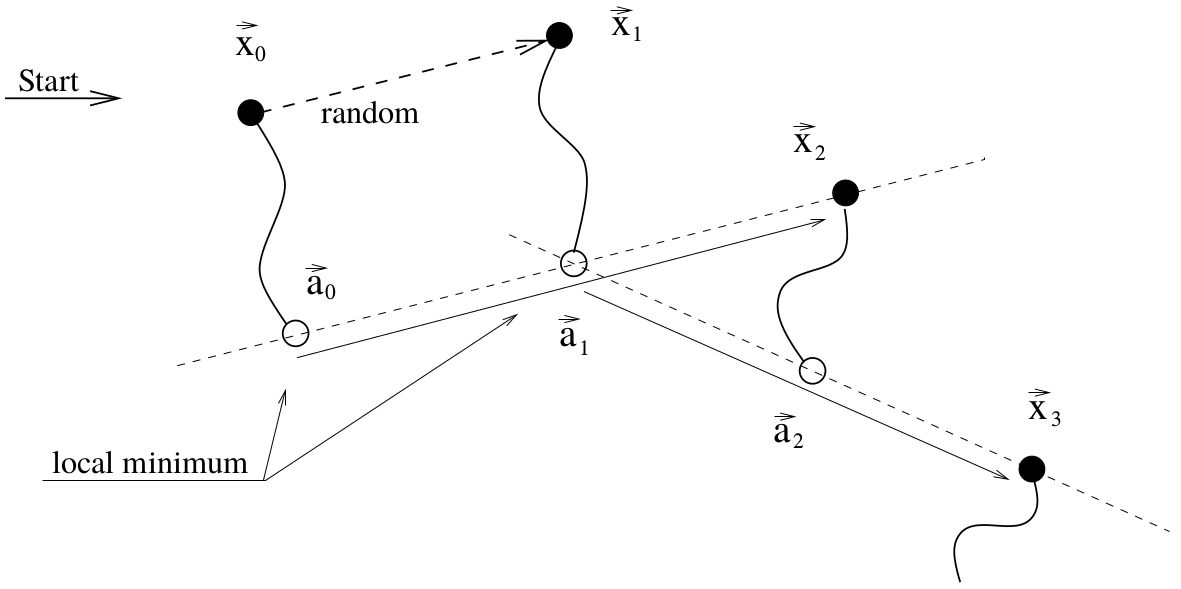
\includegraphics[width=1\textwidth]{img/17/algo_g-c}
    \end{center}
  \end{frame}

  \begin{frame}{Algorytm Gelfanda-Cetlina (stepping m.)}
    \begin{enumerate}
      \item z $\vec{x_{0}}$ -- lokalna minimalizacja --
      min. w $\vec{a_{0}}$
      \item z $\vec{x_{0}}$ -- długi, losowy krok do $\vec{x_{1}}$
      \item z $\vec{x_{1}}$ -- lokalna minimalizacja --
      min. w $\vec{a_{1}}$
      \item długi krok (precipitous step) wzdłuż
      $\vec{a_{1}} - \vec{a_{0}}$ do $\vec{x_{2}}$
      \item z $\vec{x_{2}}$ -- lokalna minimalizacja --
      min. w $\vec{a_{2}}$
      \item długi krok wzdłuż $\vec{a_{2}} - \vec{a_{1}}$ \dots itd.
    \end{enumerate}
  \end{frame}

  \begin{frame}{Algorytm Gelfanda-Cetlina (stepping m.)}
    \begin{block}{Metoda jest nielokalna}
      Przeszukiwanie zarówno w kierunku rosnących jak i
      malejących wartości $F(x)$, z preferencją w kierunku
      malejących (przewaga szukania nad zbieżnością).\\
      \emph{O jakości} decyduje wybór \emph{"precipitous~step"}
      -- zwykle met. prób i błędów.\\
      \textbf{Wada} - brak kryterium zatrzymania.
    \end{block}

    \begin{block}{Kryteria}
      \begin{itemize}
        \item czas obliczeń
        \item liczba wywołań $F(x)$
        \item uzyskanie $F(x)$ mniejszej od pewnej zadanej
        wartości
        \item "zatoczenie koła" (trudne stwierdzenie)
      \end{itemize}
    \end{block}
  \end{frame}

  \subsection{Metoda Goldstein'a-Price'a}

  \begin{frame}{Metoda Goldstein'a-Price'a}
    \begin{itemize}
      \item ładna i prosta
      \item oparta na własnościach analitycznych $F(x)$
    \end{itemize}
    W pobliżu lokalnego minimum $x_{1}{,}, F(x)$:
    \begin{displaymath}
      F(\vec{x})=F(\vec{x_{1}}) \underbrace{+}_{(!)}
      \frac{1}{2} \cdot (\vec{x} - \vec{x_{1}})^T \cdot
      G \cdot (\vec{x} - \vec{x_{1}}) +
      \underbrace{h.t.}_{\text{\emph{higher therms}}}
    \end{displaymath}
    (!) -- zanikły pierwsze pochodne!\\
    \smallskip
    Człony z 3-cią i wyższymi pochodnymi zawierają informacje
    o pozostałych minimach.
  \end{frame}

  \begin{frame}
    Usunięcie minimum w $x_{1}$ -- przez transformację:
    \begin{displaymath}
      F(\vec{x_{1}}{,}\vec{x}) =
      \frac{2 \cdot \left[ F(\vec{x}) - F(\vec{x_{1}}) \right]}
      {(\vec{x} - \vec{x_{1}})^T \cdot G \cdot (\vec{x} - \vec{x_{1}})} =
      1 + h.t.
    \end{displaymath}
    G -- dodatnio określona (bo -- w minimum) $\Rightarrow$
    w mianowniku forma kwadratowa zawsze dodatnia, czyli
    po znalezieniu min $F_{1}(x)$ mamy:
    \begin{itemize}
      \item gdy $F_{1}(x) < 0 \to$ znaleziono lepsze
      (głębsze) minimum
      \item gdy $F_{1}(x) > 0 \to$ znaleziono inne minimum
      lokalne, nie lepsze od tego w $x_{1}$; $\Rightarrow$
      z tego punktu $(x_{2}) \Rightarrow F_{2}$ (związane z
      $F_{1}$ tak, jak $F_{1}$ z $F$)
    \end{itemize}
    \begin{alertblock}{Uwaga}
      Metoda ta grozi zapętleniem, powtarzać
      ja nie więcej niż kilka razy.
    \end{alertblock}
  \end{frame}

  \subsection{Uwagi końcowe}
  \begin{frame}{Uwagi końcowe}
    \begin{itemize}
      \item nie ma \emph{uniwersalnych} metod
      minimalizacji tj.:
      \begin{itemize}
        \item[--] wszystkie funkcje
        \item[--] wszystkie obszary danej funkcji
      \end{itemize}
      \item zalecane: używanie różnych metod
      \item stopniowe zbliżanie się do minimum $\to$
      kolejno:
      \begin{itemize}
        \item[--] metody Monte Carlo
        \item[--] metody simplex / metoda Rosebrocka
        (bezgradientowa)
        \item[--] metody gradientowe
      \end{itemize}
      \item wykorzystać dostępną informację o $F(x)$
      \item ważna: zadania z ograniczeniami (funkcje kary)
    \end{itemize}
  \end{frame}

  \begin{frame}{Uwagi końcowe}
    \begin{itemize}
      \item powszechnie używany pakiet minimalizacyjny:
      F.~James, M.~Roos: MINUIT, CERN Program Library
      long write up D506 (516) $\Rightarrow$ zapoznać się!
      \item głębsze wprowadzenie w zagadnienia minimalizacji
      R.~Wit: "Metody programowania nieliniowego" WNT, Warszawa
      1986
      \item alternatywne
      \begin{itemize}
        \item Simulated annealing
        \item Genetic algorithms
      \end{itemize}
    \end{itemize}
  \end{frame}
